

\begin{frame}{Requerimientos de biblioteca de Stack} 
    \begin{itemize}
        \item Protocolo LIFO
        \item El tamano de el stack debe ser configurable por el usuario
    \end{itemize}
\end{frame}

\begin{frame}{Primer Acercamiento} 
    \inputminted[mathescape,
               linenos,
               numbersep=2pt,
               frame=lines,
               bgcolor=White,
               fontsize=\small,
               linenos,
               framesep=1mm]{c++}
               {\MyCode/testSkeleton.cpp} 
\end{frame}

\begin{frame}{Primer Acercamiento, salida} 
\begin{center}
\begin{tikzpicture}[]
\node[] at (0mm,0mm){
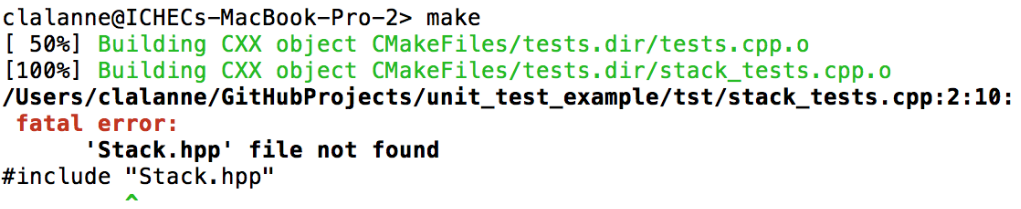
\includegraphics[height=25mm]{\MyFigures/output2.png}\hspace{5mm}
           };
        \end{tikzpicture}
    \end{center}
\end{frame}


\begin{frame}{Primer Acercamiento, implementando} 
    \inputminted[mathescape,
               linenos,
               numbersep=2pt,
               frame=lines,
               bgcolor=White,
               fontsize=\small,
               linenos,
               framesep=1mm]{c++}
               {\MyCode/stack0.cpp} 
\end{frame}


\begin{frame}{Creando el primer exito} 
    \inputminted[mathescape,
               linenos,
               numbersep=2pt,
               frame=lines,
               bgcolor=White,
               fontsize=\tiny,
               linenos,
               framesep=1mm]{c++}
               {\MyCode/stack1.cpp} 
\end{frame}

\begin{frame}{Creando el primer exito, salida} 
\begin{center}
\begin{tikzpicture}[]
\node[] at (0mm,0mm){
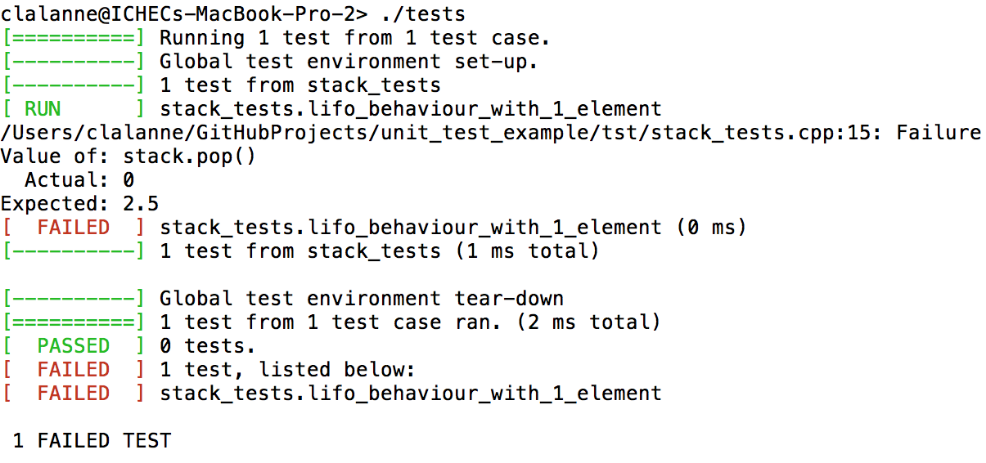
\includegraphics[height=40mm]{\MyFigures/output3.png}\hspace{5mm}
           };
        \end{tikzpicture}
    \end{center}
\end{frame}

\begin{frame}{Algo util} 
    \inputminted[mathescape,
               linenos,
               numbersep=2pt,
               frame=lines,
               bgcolor=White,
               fontsize=\tiny,
               linenos,
               framesep=1mm]{c++}
               {\MyCode/test1.cpp} 
\end{frame}

\begin{frame}{Algo util, salida} 
\begin{center}
\begin{tikzpicture}[]
\node[] at (0mm,0mm){
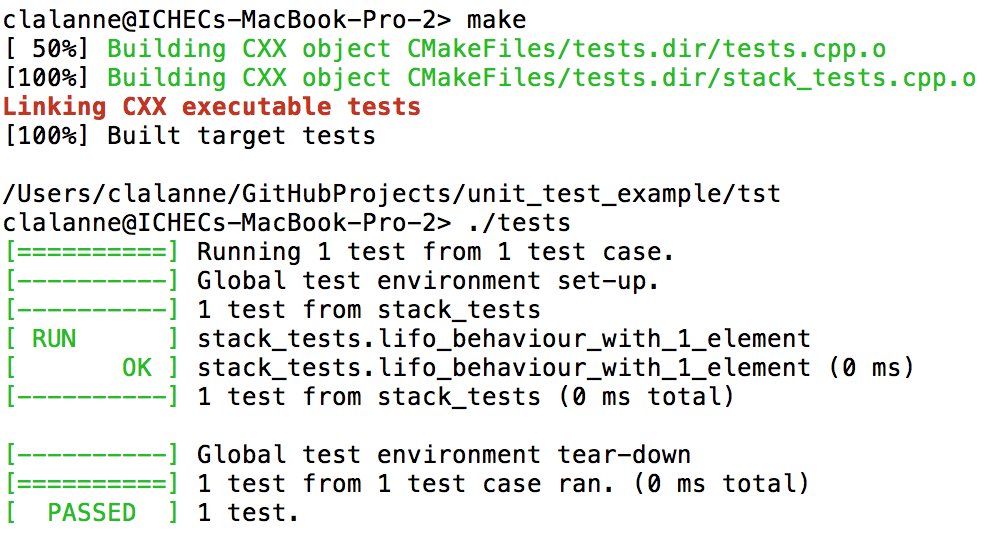
\includegraphics[height=40mm]{\MyFigures/output4.png}\hspace{5mm}
           };
        \end{tikzpicture}
    \end{center}
\end{frame}

\begin{frame}{Tomando Forma} 
    \inputminted[mathescape,
               linenos,
               numbersep=2pt,
               frame=lines,
               bgcolor=White,
               fontsize=\tiny,
               linenos,
               framesep=1mm]{c++}
               {\MyCode/stack2.cpp} 
\end{frame}

\begin{frame}{Tomando Forma, salida} 
\begin{center}
\begin{tikzpicture}[]
\node[] at (0mm,0mm){
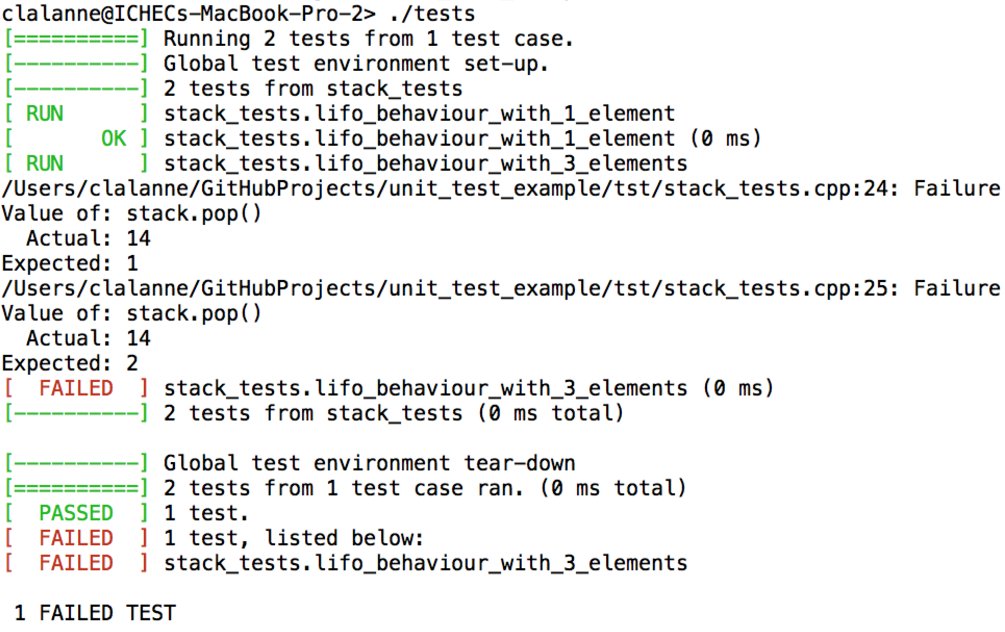
\includegraphics[height=60mm]{\MyFigures/output5.png}\hspace{5mm}
           };
        \end{tikzpicture}
    \end{center}
\end{frame}

\begin{frame}{Biblioteca Stack} 
    \begin{itemize}
        \item Casos bordes
    \end{itemize}
\end{frame}

\begin{frame}{POP de un stack vacio} 
    \inputminted[mathescape,
               linenos,
               numbersep=2pt,
               frame=lines,
               bgcolor=White,
               fontsize=\tiny,
               linenos,
               framesep=1mm]{c++}
               {\MyCode/emptyStackTest.cpp} 
\end{frame}

\begin{frame}{pasando, salida} 
\begin{center}
\begin{tikzpicture}[]
\node[] at (0mm,0mm){
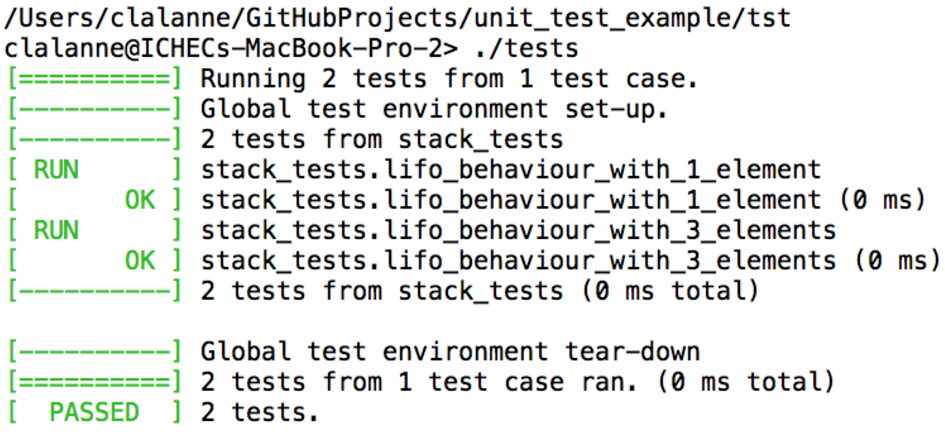
\includegraphics[height=20mm]{\MyFigures/output6.png}\hspace{5mm}
           };
        \end{tikzpicture}
    \end{center}
\end{frame}

\begin{frame}{POP de un stack vacio, implementacion} 
    \inputminted[mathescape,
               linenos,
               numbersep=2pt,
               frame=lines,
               bgcolor=White,
               fontsize=\tiny,
               linenos,
               framesep=1mm]{c++}
               {\MyCode/EmptyStackException.cpp} 
\end{frame}

\begin{frame}{POP de un stack vacio, salida} 
\begin{center}
\begin{tikzpicture}[]
\node[] at (0mm,0mm){
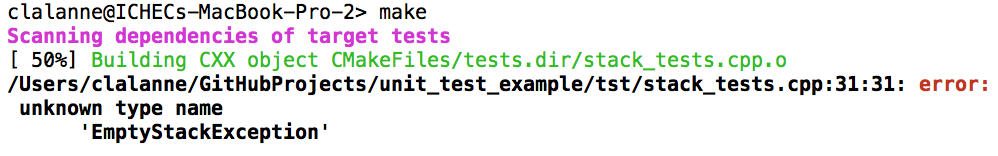
\includegraphics[height=15mm]{\MyFigures/output7.png}\hspace{5mm}
           };
        \end{tikzpicture}
    \end{center}
\end{frame}

\begin{frame}{POP de un stack vacio, implementacion stack} 
    \inputminted[mathescape,
               linenos,
               numbersep=2pt,
               frame=lines,
               bgcolor=White,
               fontsize=\tiny,
               linenos,
               framesep=1mm]{c++}
               {\MyCode/stack3.cpp} 
\end{frame}

\begin{frame}{POP de un stack vacio, salida} 
\begin{center}
\begin{tikzpicture}[]
\node[] at (0mm,0mm){
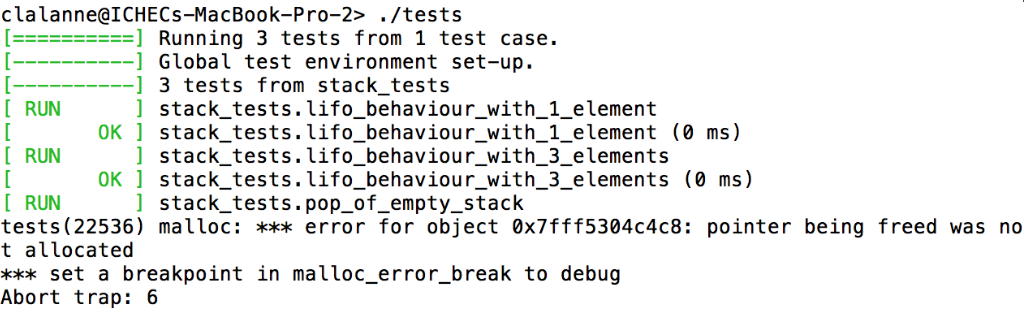
\includegraphics[height=40mm]{\MyFigures/output8.png}\hspace{5mm}
           };
        \end{tikzpicture}
    \end{center}
\end{frame}

\begin{frame}{Mas casos de borde} 
    \begin{itemize}
        \item Limite de tamano de el stack, tiene que ser configurable por el usuario
    \end{itemize}
\end{frame}

\begin{frame}{Tamano configurable} 
    \inputminted[mathescape,
               linenos,
               numbersep=2pt,
               frame=lines,
               bgcolor=White,
               fontsize=\tiny,
               linenos,
               framesep=1mm]{c++}
               {\MyCode/configurableSizeTest.cpp} 
\end{frame}

\begin{frame}{Tamano configurable, salida} 
\begin{center}
\begin{tikzpicture}[]
\node[] at (0mm,0mm){
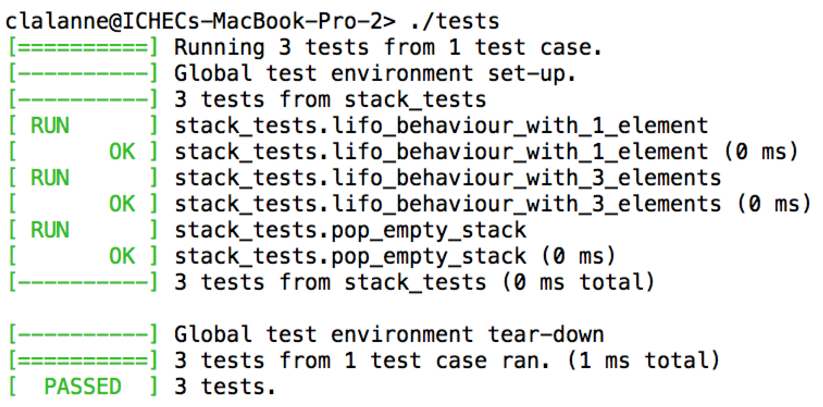
\includegraphics[height=40mm]{\MyFigures/output9.png}\hspace{5mm}
           };
        \end{tikzpicture}
    \end{center}
\end{frame}

\begin{frame}{Tamano configurable, implementacion} 
    \inputminted[mathescape,
               linenos,
               numbersep=2pt,
               frame=lines,
               bgcolor=White,
               fontsize=\tiny,
               linenos,
               framesep=1mm]{c++}
               {\MyCode/stack4.cpp} 
\end{frame}

\begin{frame}{Tamano configurable, salida} 
\begin{center}
\begin{tikzpicture}[]
\node[] at (0mm,0mm){
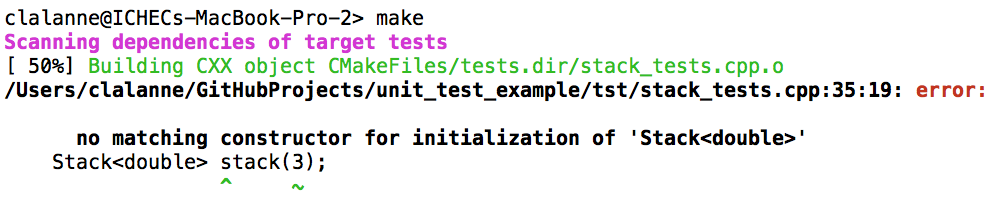
\includegraphics[height=20mm]{\MyFigures/output10.png}\hspace{5mm}
           };
        \end{tikzpicture}
    \end{center}
\end{frame}

\begin{frame}{Excede limite de tamano} 
    \inputminted[mathescape,
               linenos,
               numbersep=2pt,
               frame=lines,
               bgcolor=White,
               fontsize=\tiny,
               linenos,
               framesep=1mm]{c++}
               {\MyCode/ExceedsStackSizeException.cpp} 
\end{frame}

\begin{frame}{Importo codigo} 
    \inputminted[mathescape,
               linenos,
               numbersep=2pt,
               frame=lines,
               bgcolor=White,
               fontsize=\tiny,
               linenos,
               framesep=1mm]{c++}
               {\MyCode/finalImports.hpp} 
\end{frame}

\begin{frame}{Importo codigo, salida} 
\begin{center}
\begin{tikzpicture}[]
\node[] at (0mm,0mm){
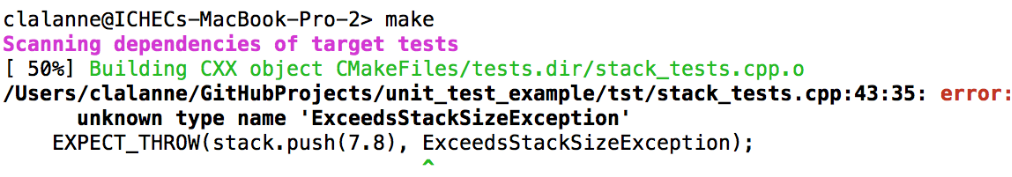
\includegraphics[height=20mm]{\MyFigures/output11.png}\hspace{5mm}
           };
        \end{tikzpicture}
    \end{center}
\end{frame}

\begin{frame}{Codigo final} 
    \inputminted[mathescape,
               linenos,
               numbersep=2pt,
               frame=lines,
               bgcolor=White,
               fontsize=\tiny,
               linenos,
               framesep=1mm]{c++}
               {\MyCode/stack5.cpp} 
\end{frame}

\begin{frame}{Codigo final, salida} 
\begin{center}
\begin{tikzpicture}[]
\node[] at (0mm,0mm){
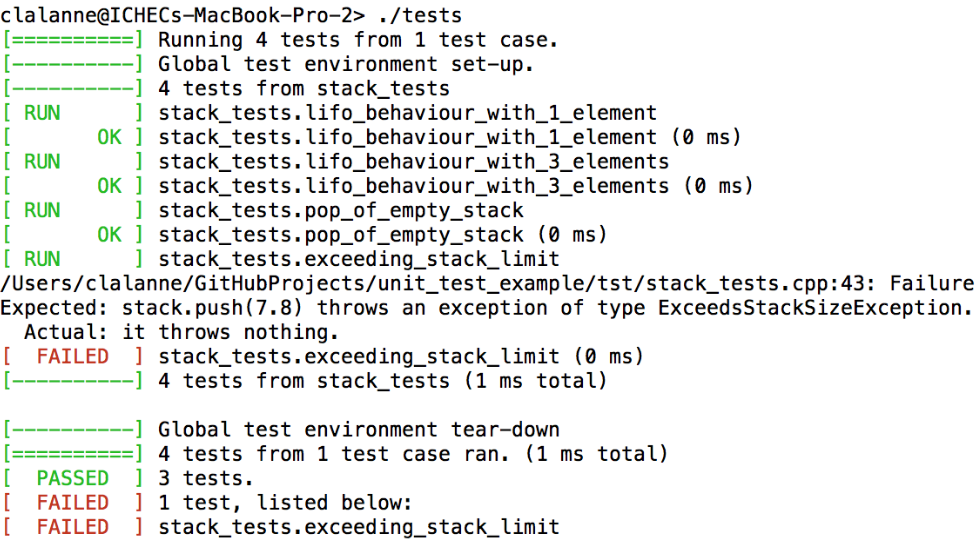
\includegraphics[height=40mm]{\MyFigures/output12.png}\hspace{5mm}
           };
        \end{tikzpicture}
    \end{center}
\end{frame}

\begin{frame}{Codigo final, salida} 
\begin{center}
\begin{tikzpicture}[]
\node[] at (0mm,0mm){
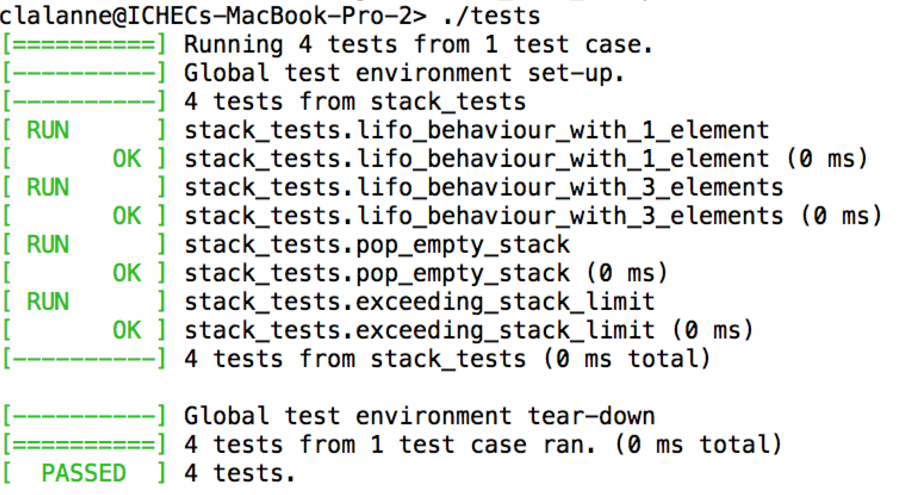
\includegraphics[height=40mm]{\MyFigures/output13.png}\hspace{5mm}
           };
        \end{tikzpicture}
    \end{center}
\end{frame}

\begin{frame}{Todos los tests} 
    \inputminted[mathescape,
               linenos,
               numbersep=2pt,
               frame=lines,
               bgcolor=White,
               fontsize=\tiny,
               linenos,
               framesep=1mm]{c++}
               {\MyCode/allTests.cpp} 
\end{frame}

\begin{frame}{Ciclo TDD}
\begin{center}
\begin{tikzpicture}[]
\node[] at (0mm,0mm){
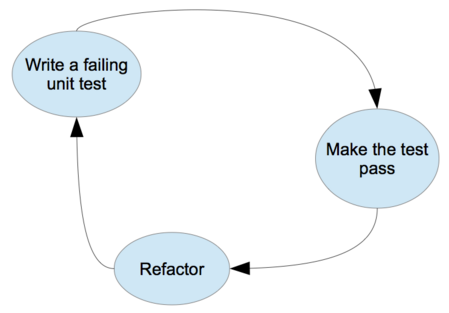
\includegraphics[height=40mm]{\MyFigures/tddCycle.png}\hspace{5mm}
           };
        \end{tikzpicture}
    \end{center}
\end{frame}

\begin{frame}{Test Driven Development} 
    \begin{itemize}
        \item Rapida y continua retro-alimentacion
        \item TDD abilita refactoring
        \item Lecciones aprendidas, experiencias ganadas no se pierden, quedan en los tests
    \end{itemize}
\end{frame}

\begin{frame}{Test Driven Development} 
    \begin{itemize}
        \item Esto trae consigo desarrollo de software incremental e iterativo
        \item El codigo final generalmente esta bien disenado y 
            \textcolor{red}{tiene tests unitarios!!!!}
        \item No es la respuesta a todos los problemas en desarrollo de software, pero
            definitivamente una mejor al hack, hack, hack and fix
    \end{itemize}
\end{frame}
